\documentclass{standalone}
\usepackage{tikz}
\usepackage{tikz-network}
\usepackage{subcaption}
\usepackage{graphicx}
% \usetikzlibrary{graphs, graphdrawing, positioning, quotes}
\usepackage{color}
\definecolor{lightblue}{RGB}{158,202,225}
\begin{document}
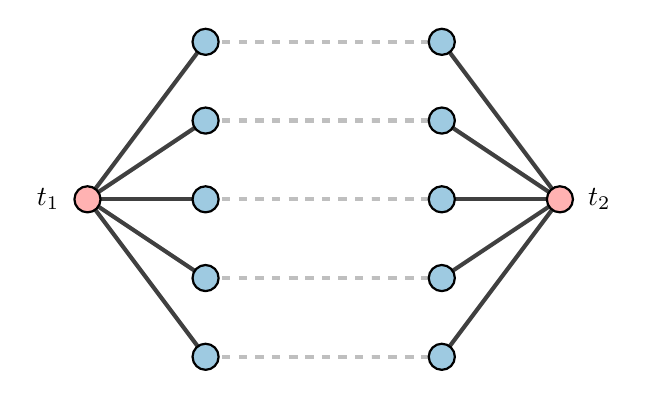
\begin{tikzpicture}
        \coordinate (t1) at (-3,0);
        \coordinate (t2) at (3,0);
        \coordinate (l1) at (-1.5,2);
        \coordinate (l2) at (-1.5,1);
        \coordinate (l3) at (-1.5,0);
        \coordinate (l4) at (-1.5,-1);
        \coordinate (l5) at (-1.5,-2);

        \coordinate (r1) at (1.5,2);
        \coordinate (r2) at (1.5,1);
        \coordinate (r3) at (1.5,0);
        \coordinate (r4) at (1.5,-1);
        \coordinate (r5) at (1.5,-2);

        \node[draw,circle,fill=red!30,thick,minimum size=8pt] (CircleNode) at (t1){};
        \node at (-3.5,0) {$t_1$};
        \node at (3.5,0) {$t_2$};
        \node[draw,circle,fill=red!30,thick,minimum size=8pt] (CircleNode) at (t2){};
        \node[draw,circle,fill=lightblue,thick,minimum size=8pt] (CircleNode) at (l1){};
        \node[draw,circle,fill=lightblue,thick,minimum size=8pt] (CircleNode) at (l2){};
        \node[draw,circle,fill=lightblue,thick,minimum size=8pt] (CircleNode) at (l3){};
        \node[draw,circle,fill=lightblue,thick,minimum size=8pt] (CircleNode) at (l4){};
        \node[draw,circle,fill=lightblue,thick,minimum size=8pt] (CircleNode) at (l5){};
        \node[draw,circle,fill=lightblue,thick,minimum size=8pt] (CircleNode) at (r1){};
        \node[draw,circle,fill=lightblue,thick,minimum size=8pt] (CircleNode) at (r2){};
        \node[draw,circle,fill=lightblue,thick,minimum size=8pt] (CircleNode) at (r3){};
        \node[draw,circle,fill=lightblue,thick,minimum size=8pt] (CircleNode) at (r4){};
        \node[draw,circle,fill=lightblue,thick,minimum size=8pt] (CircleNode) at (r5){};
        \Edge(t1)(l1)
        \Edge(t1)(l2)
        \Edge(t1)(l3)
        \Edge(t1)(l4)
        \Edge(t1)(l5)
        \Edge(t2)(r1)
        \Edge(t2)(r2)
        \Edge(t2)(r3)
        \Edge(t2)(r4)
        \Edge(t2)(r5)
        \Edge[style={dashed},color=gray!50](l1)(r1)
        \Edge[style={dashed},color=gray!50](l2)(r2)
        \Edge[style={dashed},color=gray!50](l3)(r3)
        \Edge[style={dashed},color=gray!50](l4)(r4)
        \Edge[style={dashed},color=gray!50](l5)(r5)
    \end{tikzpicture}
\end{document}